\newcommand{\doctitle}{计算机系统结构第三次作业}
\documentclass[oneside,a4paper]{article}

\usepackage{parskip}
\usepackage{subfigure}
% \usepackage{geometry}
\usepackage{amsmath}
\usepackage[dvipdfm]{graphicx} 
\usepackage{amsthm,amssymb}
\usepackage{tikz}
\usepackage{fontspec,xltxtra,xunicode}


\usepackage{fancyvrb}
% \usepackage{fancybox}
\usepackage{listings}
\lstset{numbers=left, 
  numberstyle=\scriptsize,
  frame=single,
  flexiblecolumns=false,
  language=,
  texcl=true,
  escapechar=\%,
  basicstyle=\ttfamily\small, 
  breaklines=true,
  extendedchars=true,
  showstringspaces=false,
  keywordstyle=\bfseries}

% \usepackage{indentfirst} 


\usepackage{pstricks} 
\usepackage[dvipdfm,a4paper,
hyperindex=true,
backref=section,
bookmarks=true,
bookmarksnumbered=true,
pdfpagemode=UseOutlines,
pdffitwindow=true,
linkbordercolor=white, % 链接边框设置为白色
citebordercolor=white, % 链接边框设置为白色
urlbordercolor=white]{hyperref}
          

% \DefineShortVerb{\|}

\usepackage[CJKtextspaces,CJKmathspaces,CJKchecksingle]{xeCJK}
\setCJKmainfont[BoldFont={Adobe Heiti Std}, ItalicFont={Adobe Kaiti Std}]{Adobe Song Std}
\setCJKmonofont{Adobe Fangsong Std}
\xeCJKsetcharclass{"0}{"2E7F}{0}
\xeCJKsetcharclass{"2E80}{"FFFF}{1}

\setmainfont[Mapping=tex-text]{Linux Libertine O}
\setsansfont[Mapping=tex-text]{Linux Biolinum O} 
\setmonofont{Courier 10 Pitch} 
\punctstyle{quanjiao} 


\renewcommand{\figurename}{图}
\renewcommand{\tablename}{表}
\renewcommand{\lstlistingname}{程序清单}

\newenvironment{solve}{%
  \settowidth{\leftskip}{\textit{解:}\ }%
  \makebox[0pt][r]{\textit{解:}\ }%
  \ignorespaces}{\qed\par\ignorespacesafterend}

\author{\textsc{Computer Science} 0813\\谢松 U200814454}
\title{\doctitle}
\hypersetup{
  pdftitle={\doctitle},
  pdfauthor={谢松},
  pdfsubject={\doctitle}}
\usepackage{booktabs}

\begin{document}


\maketitle

%%% Local Variables: 
%%% mode: latex
%%% TeX-master: t
%%% End: 


\section{Ex 3.11}

\begin{solve}
  \begin{enumerate}
  \item 无Forwarding, 排空流水线的情况下的时空图

    \begin{flushleft}
      \footnotesize
      \begin{tabular}{@{~}lc@{~}c@{~}c@{~}c@{~}c@{~}c@{~}c@{~}c@{~}c@{~}c@{~}c@{~}c@{~}c@{~}c@{~}c@{~}c@{~}c@{~}c@{~}c@{~}c@{~}c@{~}c@{~}c@{~}}
        指令
        & 1  & 2  & 3  & 4  & 5  & 6  & 7  & 8  & 9  & 10 & 11 & 12 & 13 & 14 & 15 & 16 & 17 & 18 & 19 & 20 & 21 & 22 & 23 \\
        \texttt{LW}     & IF & ID & EX & M  & WB \\
        \texttt{DADDIU} &    & IF & S  & S  & ID & EX & M  & WB \\
        \texttt{SW}     &    &    &    &    & IF & S  & S  & ID & EX & M  & WB \\
        \texttt{DADDIU} &    &    &    &    &    &    &    & IF & ID & EX & M  & WB \\
        \texttt{DSUB}   &    &    &    &    &    &    &    &    & IF & S  & S  & S  & ID & EX & M  & WB \\
        \texttt{BNEZ}   &    &    &    &    &    &    &    &    &    &    &    &    & IF & S  & S  & ID & EX & M  & WB \\
        \texttt{LW}     &    &    &    &    &    &    &    &    &    &    &    &    &    &    &    & IF & S  & S  & IF & ID & EX & M  & WB \\
      \end{tabular}
    \end{flushleft}

    在这种情况下, 上述循环需要$15\times{}99 + 4 = 1489$个时钟周期.

    
  \item 正常Forwarding, 分支预测失败情况下的时空图

    \begin{flushleft}
      \footnotesize
      \begin{tabular}{@{~}lc@{~}c@{~}c@{~}c@{~}c@{~}c@{~}c@{~}c@{~}c@{~}c@{~}c@{~}c@{~}c@{~}c@{~}}
        指令
        & 1  & 2  & 3  & 4  & 5  & 6  & 7  & 8  & 9  & 10 & 11 & 12 & 13 & 14 \\
        \texttt{LW}     & IF & ID & EX & M  & WB \\
        \texttt{DADDIU} &    & IF & S  & ID & EX & M  & WB \\
        \texttt{SW}     &    &    &    & IF & ID & EX & M  & WB \\
        \texttt{DADDIU} &    &    &    &    & IF & ID & EX & M  & WB \\
        \texttt{DSUB}   &    &    &    &    &    & IF & ID & EX & M  & WB \\
        \texttt{BNEZ}   &    &    &    &    &    &    & IF & S  & ID & EX & M  & WB \\
        \texttt{LW}     &    &    &    &    &    &    &    & IF & S  & IF & ID & EX & M  & WB \\
      \end{tabular}
    \end{flushleft}

    在这种情况下, 上述循环需要$9\times{}99 + 3 = 894$个时钟周期.
    
  \item 正常Forwarding, 单周期延迟分支, 调度后的代码如程序清单~\ref{lst:3-11-re}所示.

    \lstinputlisting[language=, caption=重调度后的代码, label={lst:3-11-re}]{3-11-re.s}
    
    \begin{flushleft}
      \footnotesize
      \begin{tabular}{@{~}lc@{~}c@{~}c@{~}c@{~}c@{~}c@{~}c@{~}c@{~}c@{~}c@{~}c@{~}}
        指令
        & 1  & 2  & 3  & 4  & 5  & 6  & 7  & 8  & 9  & 10 & 11 \\
        \texttt{LW}     & IF & ID & EX & M  & WB \\
        \texttt{DADDIU} &    & IF & ID & EX & M  & WB \\
        \texttt{DSUB}   &    &    & IF & ID & EX & M  & WB \\
        \texttt{DADDIU} &    &    &    & IF & ID & EX & M  & WB \\
        \texttt{BNEZ}   &    &    &    &    & IF & ID & EX & M  & WB \\
        \texttt{SW}     &    &    &    &    &    & IF & ID & EX & M  & WB \\
        \texttt{LW}     &    &    &    &    &    &    & IF & ID & EX & M  & WB \\
      \end{tabular}
    \end{flushleft}

    在这种情况下, 上述循环需要$6\times{}99 + 4 = 598$个时钟周期.
  \end{enumerate}
\end{solve}
\section{Lab 2}

\begin{solve}
  \begin{enumerate}
  \item 模拟程序代码见程序清单~\ref{lst:3-11}.

    \lstinputlisting[caption={Ex 3.11 模拟程序清单}, label=lst:3-11]{3-11.s}
  \item 时钟周期比较结果如下所示:
    
    \begin{tabular}{lccc}
      \toprule
      时钟周期   & (1)  & (2) & (3) \\\midrule
      人工计算   & 1489 & 894 & 598 \\
      WinMIPS64 & 1492 & 897 & 601 \\\bottomrule
    \end{tabular}
    
  \item 人工计算和WinMIPS64模拟的结果有差异, 差异的原因是在模拟的过程
    中, 需要加入指令设置寄存器R2, R3的初值, 并且额外加了一
    条\texttt{halt}指令, 因此人工计算的时钟周期数比模拟的结果少3个时钟
    周期.
  \item 对3种不同条件的流水线模拟截图及分析如下:
    \begin{enumerate}
    \item 无Forwarding的流水线时空图如图~\ref{fig:3-11-1}所示. 
      
      \begin{figure}[!h]
        \centering
        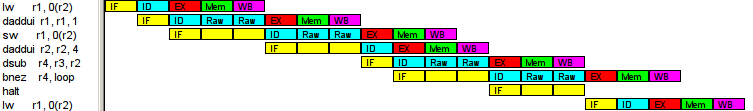
\includegraphics[width=0.9\textwidth]{img/1.png}
        \caption{无Forwarding的流水线时空图}
        \label{fig:3-11-1}
      \end{figure}

      从图中可以看到在无Forwarding的情况下, RAW冲突频繁发生.
      
    \item 有Forwarding的流水线时空图如图~\ref{fig:3-11-2}所示. 
      
      \begin{figure}[!h]
        \centering
        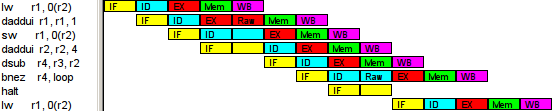
\includegraphics[width=0.8\textwidth]{img/2.png}
        \caption{有Forwarding的流水线时空图}
        \label{fig:3-11-2}
      \end{figure}

      从图中可以看到在有Forwarding的情况下, 访存后立即使用数据带来的冲
      突依然无法解决, 必须引入一个时钟周期的Stall. 而且对于这样的用于循
      环的分支,预测失败不是好策略.
      
    \item 有Forwarding, 延迟分支的流水线时空图如图~\ref{fig:3-11-3}所
      示. 
      
      \begin{figure}[!h]
        \centering
        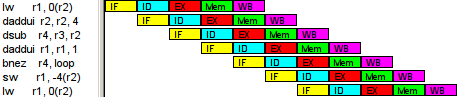
\includegraphics[width=0.65\textwidth]{img/3.png}
        \caption{有Forwarding, 延迟分支的流水线时空图}
        \label{fig:3-11-3}
      \end{figure}

      从图中可以看到, 经过重新调度后的代码在流水线中可以不用加入任
      何Stall而顺利执行, 这样代码的执行效率达到最高.
    \end{enumerate}
    
  \end{enumerate}
\end{solve}

\section{Ex 5.8}

\begin{solve}
  \begin{enumerate}
  \item 程序执行的CPI

    \begin{align*}
      CPI &= 1 + 15\% \times{} (10\% \times{} 3 + 90\% \times{} (10\%\times{}4)) \\
      &= 1.099
    \end{align*}
  \item 若采用2周期延迟的分支处理, 那么程序执行的CPI

    \begin{align*}
      CPI' &= 1 + 15\% \times{} 2\\
      &= 1.3,
    \end{align*}
    大于使用BTB的CPI. 因此, 使用BTB能使程序执行速度更快.
  \end{enumerate}
\end{solve}

\section{Ex 5.9}

\begin{solve}
  设单条无条件转移指令的延迟为$x$, 则有:
  \begin{displaymath}
    1+5\%\times{}x=1.1.
  \end{displaymath}

  解之, 得 $x=2$.

  当分支目标缓冲命中时, 无条件转移指令的延迟为0. 故, 程序的CPI:
  \begin{align*}
    CPI &= 1 + 2 \times 5\% \times (1 - 90\% ) \\
    &= 1.01
  \end{align*}
\end{solve}

\section{Ex 5.11}

\begin{solve}
  \begin{enumerate}
  \item 标量流水处理机
    
    \begin{center}
      \begin{tikzpicture}[scale=.7]
        \draw[->] (0, 0) -- (15.3, 0) node[below] {时间} coordinate(x axis);
        \draw[->] (0, 0) -- (0, 4) node[left] {阶段} coordinate(y axis);
        \draw[step=1, help lines](0, 0) grid (14, 3);
        \foreach \x in {0, ..., 14}
        \draw (\x, 0) node[below] {\x};
        \draw (0, 0.5) node[left] {取指};
        \draw (0, 1.5) node[left] {分析};
        \draw (0, 2.5) node[left] {执行};
        \foreach \y in {0, 1, 2}{
          \foreach \x in {0, ..., 11}
          \filldraw[color=blue, fill=blue!20, thick]
          (\x+\y, \y) -- ++(1, 0) -- ++(0,1) -- ++(-1, 0) -- cycle ;
        };
      \end{tikzpicture}
    \end{center}

    在标量流水处理机上运行给定程序, 需要$t_1 = 14\Delta{}t$时间.
  \item ILP=4的超标量处理机

    \begin{center}
      \begin{tikzpicture}[scale=.5]
        \draw[->] (0, 0) -- (6, 0) node[below] {时间} coordinate(x axis);
        \draw[->] (0, 0) -- (0, 13) node[left] {阶段} coordinate(y axis);
        \draw[step=1, help lines](0, 0) grid (5, 12);
        \foreach \x in {0, ..., 5}
        \draw (\x, 0) node[below] {\x};
        \foreach \y in {0, ..., 3}
        \draw[dashed] (0, 4*\y) -- +(-2, 0);
        \draw[<->, thick] (-1, 0) -- +(0, 4) node[midway,fill=white] {取指};
        \draw[<->, thick] (-1, 4) -- +(0, 4) node[midway,fill=white] {分析};
        \draw[<->, thick] (-1, 8) -- +(0, 4) node[midway,fill=white] {执行};
        \foreach \k in {0, 1, 2}{
          \foreach \y in {0, ..., 3}{
            \foreach \x in {0, ..., 2}
            \filldraw[color=blue, fill=blue!20, thick]
            (\k + \x , 4*\k + \y) -- ++(1, 0) -- ++(0,1) -- ++(-1, 0) -- cycle;};};        
      \end{tikzpicture}
    \end{center}
    在ILP=4的超标量处理机上运行给定程序, 需要$t_2 = 5\Delta{}t$时间. 加速比
    \begin{align*}
      S_2 &= \frac{t_1}{t_2} = \frac{14\Delta{}t}{5\Delta{}t}\\
      &= 2.8
    \end{align*}


  \item ILP=4的超长指令字处理机

    \begin{center}
      \begin{tikzpicture}[scale=.5]
        \draw[->] (0, 0) -- (6, 0) node[below] {时间} coordinate(x axis);
        \draw[->] (0, 0) -- (0, 13) node[left] {阶段} coordinate(y axis);
        \draw[step=1, help lines](0, 0) grid (5, 12);
        \foreach \x in {0, ..., 5}
        \draw (\x, 0) node[below] {\x};
        \foreach \y in {0, ..., 3}
        \draw[dashed] (0, 4*\y) -- +(-2, 0);
        \draw[<->, thick] (-1, 0) -- +(0, 4) node[midway,fill=white] {取指};
        \draw[<->, thick] (-1, 4) -- +(0, 4) node[midway,fill=white] {分析};
        \draw[<->, thick] (-1, 8) -- +(0, 4) node[midway,fill=white] {执行};
        \foreach \k in {0, 1, 2}{
          \foreach \y in {0, ..., 3}{
            \foreach \x in {0, ..., 2}
            \filldraw[color=blue, fill=blue!20, thick]
            (\k + \x , 4*\k + \y) -- ++(1, 0) -- ++(0,1) -- ++(-1, 0) -- cycle;};};          
      \end{tikzpicture}
    \end{center}
    在ILP=4的超长指令字处理机上运行给定程序, 需要$t_3 = 5\Delta{}t$时间. 加速比
    \begin{align*}
      S_3 &= \frac{t_1}{t_3} = \frac{14\Delta{}t}{5\Delta{}t}\\
      &= 2.8
    \end{align*}

  \item ILP=4的超流水处理机
    \begin{center}
      \begin{tikzpicture}[scale=.5]
        \draw[->] (0, 0) -- (7.3, 0) node[below] {时间} coordinate(x axis);
        \draw[->] (0, 0) -- (0, 13) node[left] {阶段} coordinate(y axis);
        \draw[step=1, help lines](0, 0) grid (6, 12);
        \foreach \x in {0, ..., 5}
        \draw (\x, 0) node[below] {\x};
        \foreach \y in {0, ..., 3}
        \draw[dashed] (0, 4*\y) -- +(-2, 0);
        \draw[<->, thick] (-1, 0) -- +(0, 4) node[midway,fill=white] {取指};
        \draw[<->, thick] (-1, 4) -- +(0, 4) node[midway,fill=white] {分析};
        \draw[<->, thick] (-1, 8) -- +(0, 4) node[midway,fill=white] {执行};
        \draw[dashed] (5.75, 0) -- +(0, 12);
        \draw (6, 0) node[below] {5.75};
        \foreach \y in {0, ..., 11}{
          \foreach \x in {0, ..., 2}
          \filldraw[color=blue, fill=blue!20, thick]
          (\x+0.25*\y, \y) -- ++(1, 0) -- ++(0,1) -- ++(-1, 0) -- cycle ;
        };
      \end{tikzpicture}
    \end{center}
    在ILP=4的超流水处理机上运行给定程序, 需要$t_4 = 5.75\Delta{}t$时间. 加速比
    \begin{align*}
      S_4 &= \frac{t_1}{t_4} = \frac{14\Delta{}t}{5.75\Delta{}t}\\
      &= 2.43
    \end{align*}
  \end{enumerate}
\end{solve}


\section{Ex 6.7}

\begin{solve}
  根据GCD测试方法, 在这个循环中, $a=2$, $b=2$, $c=2$,
  $d=1$. 有$\gcd(a, c) = 2$, $d-b = -1$. 由于$2\nmid{}-1$, 因此循环中
  不存在存储别名, 故不存在循环携带的真数据相关.
\end{solve}

\section{Ex 6.8}

\begin{solve}
  展开循环并对某些寄存器换名后, 得到无``空转''的代码如程序清
  单~\ref{lst:6-8}所示.

  \lstinputlisting[label=lst:6-8, caption=重调度之后完成点积运算的代码]{6-8.s}
\end{solve}


\end{document}

%%% Local Variables: 
%%% mode: latex
%%% TeX-master: t
%%% End: 


%%% Local Variables: 
%%% mode: latex
%%% TeX-master: t
%%% End: 
